%\documentclass[14pt, notes]{beamer}
\documentclass[14pt]{beamer}

%\usepackage{pgfpages}
%\setbeameroption{show notes}
%\setbeameroption{show notes on second screen=right}

%encoding
\usepackage[utf8]{inputenc}

%language
\usepackage[russian]{babel}
\usepackage{amsmath}
\usepackage{bm}
\usepackage{graphicx}
\usepackage{hyperref}
\graphicspath{{images/}}%путь к рисункам

\setbeamerfont{author in head/foot}{size=\small}
\setbeamerfont{title in head/foot}{size=\footnotesize}

\title[Моделирование динамики жидкости в сосудах]{Численное моделирование динамики жидкости в крупных кровеносных сосудах}
\date{\today}
\author[Долгов Д.А.]{Долгов Д.А.\\{\small Научный руководитель: Захаров Ю.Н.}}
\institute{Кемеровский Государственный Университет \\
    \vspace{0.7cm}
    \vspace{0.7cm}
} 
\usetheme[numbers, totalnumbers, minimal, nologo]{Statmod}
% Привычный шрифт для математических формул
\usefonttheme[onlymath]{serif}

\definecolor{statmodblue}{RGB}{100,10,30}
\definecolor{statmodsand}{RGB}{244,215,103}

\begin{document}
\maketitle

%description of the problem
\begin{frame}
\frametitle{Введение}
Рассмотрим задачу о течении крови внутри крупных сосудов с гибкими стенками. Кровь будем моделировать как вязкую, несжимаемую двухкомпонентную жидкость (плазма и форменные элементы: эритроциты, лейкоциты, тромбоциты), стенки сосуда - как поверхность заданной формы, обладающую определенной жесткостью. Стенки движутся с той же скоростью, что и жидкость.
\end{frame}

%description of the problem: schema
\begin{frame}
\frametitle{Введение}
    \begin{center}
        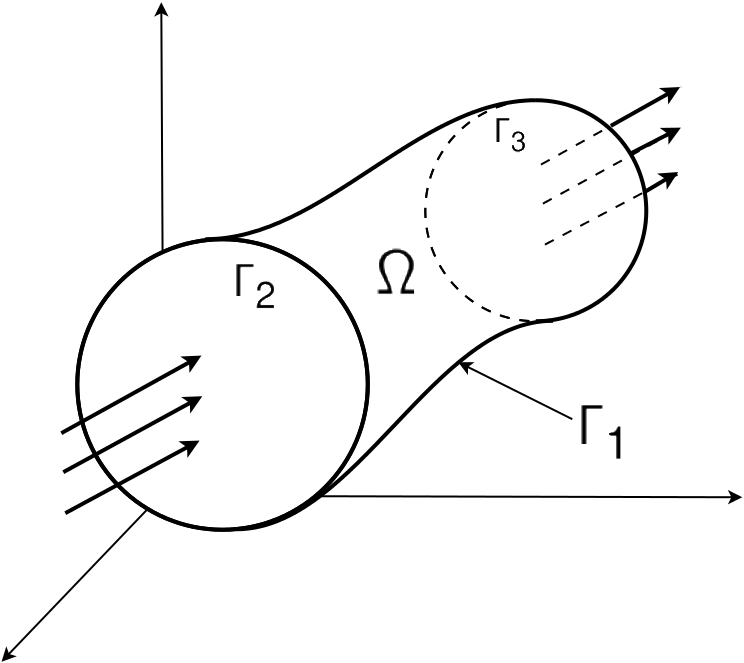
\includegraphics[width=8.5cm]{area_3d.png}
    \end{center}
\end{frame}
\note{$\Gamma_1$ - гибкие стенки, $\Gamma_2,\Gamma_3$ - вход/выход}

% navier stokes equations
\begin{frame}
\frametitle{Моделирование течения}
Система уравнений Навье-Стокса:
\begin{gather}
    \label{eq:motion}
    \rho ( \frac{\partial u}{\partial t} + u \cdot \nabla u) = - \nabla p + \nabla \cdot \sigma + f\\
    \label{eq:continuity}
    \frac{\partial \rho}{\partial t} + \nabla \cdot (\rho u) = 0 
\end{gather}
где $\sigma = \mu (\nabla u + (\nabla u)^{T})$, с начальными условиями
\begin{gather}
    u(x, y, z, t_0) = u_0
\end{gather}

\end{frame}
\note{Уравнения записаны в векторном виде, $\sigma$ - вязкий тензор напряжений}

% boundary
\begin{frame}
\frametitle{Условия на стенках}
\begin{itemize}
    \item на $\Gamma_1$ задаются условия прилипания
    \item на $\Gamma_2,\Gamma_3$ заданы значения давления $P_{int}(x, y, z),P_{out}(x, y, z)$
\end{itemize}
\end{frame}

% boundary
\begin{frame}
\frametitle{Сопротивление деформации}
В каждой точке стенки определена поверхностная сила сопротивления деформации [3]
\begin{gather}
    \label{eq:strain_energy}
    F =  \frac{\partial}{\partial s}(T \tau) + \frac{\partial^2}{\partial s^2} \Big( E \cdot I \frac{\partial^2}{\partial s^2} X \Big)
\end{gather}
\begin{gather}
    \label{eq:define_boundary_force}
    F(x, y, z, t) = k \cdot \|X(x, y, z) - X_0(x, y, z)\|
\end{gather}
\end{frame}
\note{$E$ - модуль Юнга, $I$ - момент инерции поперечного сечения, $T$ - напряжение фибры, $\tau$ - единичный тангенциальный вектор, касательный к фибре.}

% concentration
\begin{frame}
\frametitle{Концентрация}
Уравнение для расчета концентрации примеси в жидкости:
\begin{gather}
    \label{eq:concentration}
    \frac{\partial c}{\partial t} + u \cdot \nabla c = 0
\end{gather}
с начальными условиями
\begin{gather}
    c(x, y, z, 0) = c_0(x, y, z)
\end{gather}

\end{frame}

% concentration: dependencies
\begin{frame}
\frametitle{Концентрация}
Плотность и вязкость зависят от концентрации:
\begin{gather}
    \label{eq:concentration_viscosity}
    \mu = c (\mu_2 - \mu_1) + \mu_1\\
    \label{eq:concentration_density}
    \rho = c (\rho_2 - \rho_1) + \rho_1
\end{gather}

где $\mu_1, \mu_2, \rho_1, \rho_2$ - вязкости и плотности обоих компонент.
\end{frame}

% solve method 
\begin{frame}
\frametitle{Метод решения}
Будем рассматривать отдельно задачи вычисления параметров течения жидкости и параметров движения стенок сосуда и клапанов. Для этого введем в расчетной области сетки:
\begin{itemize}
    \item $\Omega_h = \Omega_h(x, y, z)$ - равномерная разнесенная сетка для расчета течения
    \item $\Gamma_h = \Gamma_h(q, r, s, t)$ - соответствует стенкам сосуда и клапанам в лагранжевых координатах
\end{itemize}

\end{frame}

% solve method: diagram
\begin{frame}
\frametitle{Метод решения}
    \begin{center}
        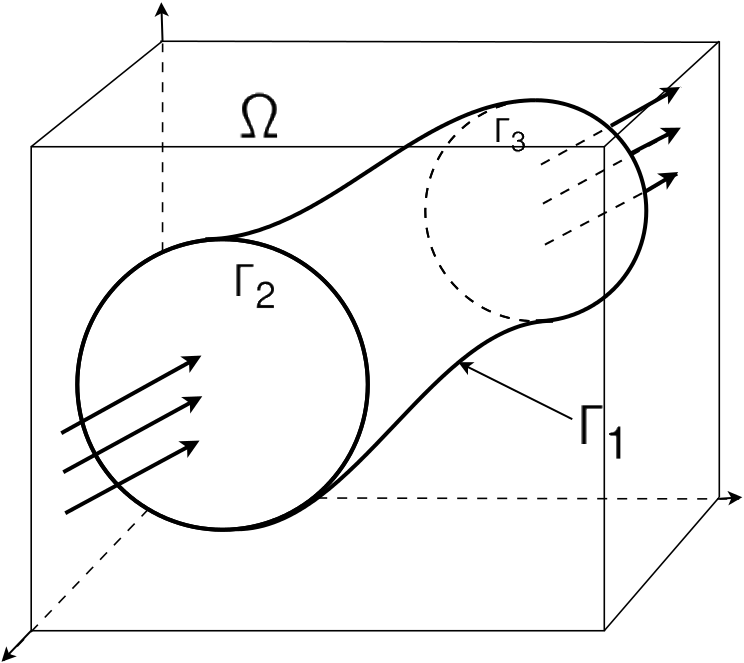
\includegraphics[width=8.5cm]{area_ibm_3d.png}
    \end{center}
\end{frame}

% solve method:immersed boundary
\begin{frame}
\frametitle{Взаимодействие}
Уравнения, описывающие взаимодействие погруженной границы и жидкости [2]:
\begin{gather}
    \label{eq:ibm_velocity}
    \frac{\partial X}{\partial t} = \int_{\Omega_h} u \cdot \delta (x - X)\; dx\; dy\; dz \\
    \label{eq:ibm_force}
    f = \int_{\Gamma_h} F \cdot \delta (x - X)\; dq\; dr\; ds
\end{gather}
и условие прилипания
\begin{gather}
    \label{eq:no_slip}
    \frac{\partial X}{\partial t} (q, r, s, t) = u(X(q, r, s, t), t)
\end{gather}
\end{frame}
\note{Заглавные символы относятся к погруженной границе, обычные - к жидкости}

% solve method:split scheme
\begin{frame}
\frametitle{Алгоритм решения}
Схема расщепления по физическим факторам:
\begin{gather}
    \label{eq:split_first}
    \frac{u^* - u^n}{\triangle t} = - (u^n \cdot \nabla) u^n + \frac{1}{\rho} \nabla \sigma + f\\
    \label{eq:split_second}
    \rho \triangle p^{n+1} - (\nabla p \cdot \nabla p^{n+1}) = \frac{\rho^2 \nabla u^*}{\triangle t}\\
    \label{eq:split_third}
    \frac{u^{n+1} - u^*}{\triangle t} = - \frac{1}{\rho} \nabla p^{n+1}
\end{gather}
где $\nabla \sigma (u^n, \mu) = \mu \triangle u^n + (\nabla \mu \cdot \nabla) u^n + (\nabla \mu \cdot J_{u^n}) $
\end{frame}
\note{
    \begin{itemize}
        \item Аппроксимируем уравнение \eqref{eq:split_first} с помощью схемы расщепления Дугласа-Рекфорда и решаем полученную систему методом прогонки
        \item Из уравнения \eqref{eq:split_second} методом бисопряженных градиентов определяем поле давления
        \item Восстанавливаем окончательное поле вектора скорости по явным формулам \eqref{eq:split_third}
    \end{itemize}
}

% solve method:ibm scheme
\begin{frame}
\frametitle{Алгоритм решения}
Интерполяция скорости на границу и распределение поверхностной силы деформации на точки жидкости:
\begin{gather}
    \label{eq:interpolation}
    U_n = \sum_{ijk}u_{ijk} \cdot D(x_{ijk} - x_n) h_{ijk}^3 \\
    \label{eq:spreading}
    f_{ijk} = \sum_n F_n \cdot D(x_{ijk} - x_n) h^2_n
\end{gather}

$D(x_n)$ соответствует $\delta(x - x_k)$, а $h_n$ - шаг сетки по погруженной границе.
\end{frame}

% solve method: force distribution scheme
\begin{frame}
\frametitle{Схема распределения силы деформации}
    \begin{center}
        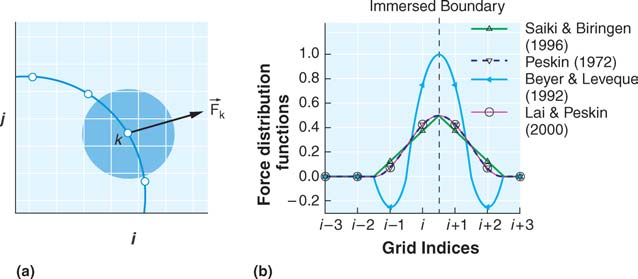
\includegraphics[width=11.5cm]{delta_function.png}
    \end{center}
\end{frame}

% totals and examples
\begin{frame}
\frametitle{Примеры}
\begin{itemize}
    \item \href{run:video/cylinder1.avi}{Деформация стенок сосуда}
    \item \href{run:video/cylinder2.avi}{Аналогичный расчет на более мелкой сетке}
\end{itemize}
\end{frame}

% totals and examples
\begin{frame}
\frametitle{Примеры}
\begin{itemize}
    \item \href{run:video/source_in_vessel.avi}{Расчет распространения примеси}
    \item \href{run:video/thrombus_in_vessel.avi}{Размыв "тромба"}
\end{itemize}
\end{frame}

\begin{frame}
\frametitle{Дополнительная информация}
    \begin{itemize}
        \item Peskin C.S., Numerical Analysis of Blood Flow in the Heart// JCP 25,220-252, (1977)
        \item Peskin C.S., The immersed boundary method// Acta numerica, 1-39, (2002)
        \item Boyce E.G. Immersed boundary model of aortic heart valve dynamics with physiological driving and loading conditions // International Journal for Numerical Methods in Biomedical Engineering. 1–29, 2011
        \item Kruger T., Introduction to the immersed boundary method, (2011)
    \end{itemize}
\end{frame}
\end{document}
